% !TEX TS-program = pdflatex
% !TEX encoding = UTF-8 Unicode

% This is a simple template for a LaTeX document using the "article" class.
% See "book", "report", "letter" for other types of document.

\documentclass[11pt]{article} % use larger type; default would be 10pt

\usepackage[utf8]{inputenc} % set input encoding (not needed with XeLaTeX)
\usepackage[spanish]{babel}
\usepackage{graphicx,wrapfig,lipsum}
%%% Examples of Article customizations
% These packages are optional, depending whether you want the features they provide.
% See the LaTeX Companion or other references for full information.

%%% PAGE DIMENSIONS
\usepackage{geometry} % to change the page dimensions
\geometry{a4paper} % or letterpaper (US) or a5paper or....
% \geometry{margin=2in} % for example, change the margins to 2 inches all round
% \geometry{landscape} % set up the page for landscape
%   read geometry.pdf for detailed page layout information

\usepackage{graphicx} % support the \includegraphics command and options
\usepackage{float}
% \usepackage[parfill]{parskip} % Activate to begin paragraphs with an empty line rather than an indent

%%% PACKAGES
\usepackage{booktabs} % for much better looking tables
\usepackage{array} % for better arrays (eg matrices) in maths
\usepackage{paralist} % very flexible & customisable lists (eg. enumerate/itemize, etc.)
\usepackage{verbatim} % adds environment for commenting out blocks of text & for better verbatim
\usepackage{subfig} % make it possible to include more than one captioned figure/table in a single float
% These packages are all incorporated in the memoir class to one degree or another...

%%% HEADERS & FOOTERS
\usepackage{fancyhdr} % This should be set AFTER setting up the page geometry
\pagestyle{fancy} % options: empty , plain , fancy
\renewcommand{\headrulewidth}{0pt} % customise the layout...
\lhead{}\chead{}\rhead{}
\lfoot{}\cfoot{\thepage}\rfoot{}

%%% SECTION TITLE APPEARANCE
\usepackage{sectsty}
\allsectionsfont{\sffamily\mdseries\upshape} % (See the fntguide.pdf for font help)
% (This matches ConTeXt defaults)

%%% ToC (table of contents) APPEARANCE
\usepackage[nottoc,notlof,notlot]{tocbibind} % Put the bibliography in the ToC
\usepackage[titles,subfigure]{tocloft} % Alter the style of the Table of Contents
\renewcommand{\cftsecfont}{\rmfamily\mdseries\upshape}
\renewcommand{\cftsecpagefont}{\rmfamily\mdseries\upshape} % No bold!

%%% END Article customizations

%%% The "real" document content comes below...

\title{Optimzing Neural Networks}
\author{Luis Moran and Diego Palomero}
%\date{} % Activate to display a given date or no date (if empty),
         % otherwise the current date is printed 

\begin{document}
\maketitle

\section{Introduction}

In this task the neural network is going to use other architectures and training algorithms to compare the results obtained with the ones in Task 2. In this case 
the Adam Algorithm will be used instead of the Gradient Descent. Additionaly, a deeper network and residual blocks will to be used too.
\section{Implementation}
Two type of architectures will to try different activation functions and learning rates on them. These architectures are:
\subsection*{Deep neural network}
For the implementation of the deep neural network with 9 hidden layers the hidden layers can be added just like in Task 2. For the Adam Optimization the optimizer Gradient Descent is changed with the class
AdamOptimizer from TensorFlow. 
\subsection*{ResNet architecture}
To create the 9 layer ResNet architecture four residual blocks are being inserted following the architecture of figure \ref{resNet}
\begin{figure}
\begin{wrapfigure}{l}{5.5cm}
    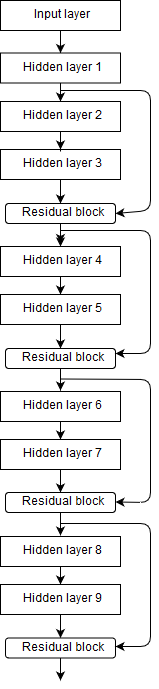
\includegraphics[scale=0.5]{images/resNetArch.PNG}
    \caption{ResNet Architecture}
    \label{resNet}
\end{wrapfigure}
\end{figure}
Each residual block  follows this function:
\[reLU(x+W_2ReLU(W_1x+b_1)+b_2)\]
referencing 1 and 2 the latest 2 layers before the residual block.
\begin{figure}
	\centering
    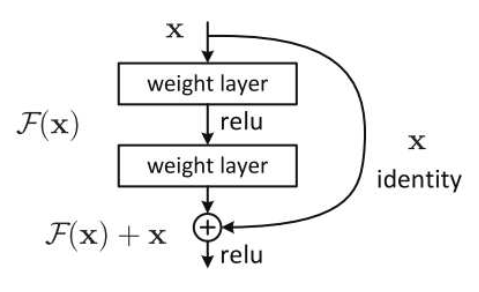
\includegraphics[scale=0.5]{images/layers.PNG}
    \caption{A residual block}
    \label{residual}
\end{figure}

Consdering the figure \ref{residual} shown in the task and the previous equation $W_1x+b_1$ is the output of the first layer, which can be called $y_1$ and in consequence 
each residual block output is: \[reLU(x+W_2y_1+b_2)\].

\section{Results}
First the 9 hidden layers architecture is tested with ReLu and tanh activation functions. Early stopping is used although the execution is not stopped (only the results saved) 
so it can be visualized in the graphics the entropy and accuracy error after the early stopping is triggered. the results represent the maximum value before the early stopping 
is triggered
\begin{table}[H]
\centering
\begin{tabular}{|l|c|c|c|}
\hline
Activation function & Learning rate & Training error & Test error \\
 \hline
 \hline
ReLu & 0.001 & 0.694 &0.555 \\
 \hline
ReLu & 0.002 & 0.744 &0.607 \\
 \hline
ReLu & 0.005 & 0.824 &0.682 \\
\hline
Tanh & 0.001 & 0.590 &0.448 \\
 \hline
Tanh & 0.002 & 0.789 & 0.632 \\
 \hline
Tanh & 0.005 & 0.077 &0.077 \\ 
\hline
\end{tabular}
\end{table}
It is noticeable how although the architecture has more layers the results are worse than in the Task 2 and they fluctuate much more in this case probably because of overfitting.
\begin{figure}[H]
  \centering
  \begin{minipage}[b]{0.4\textwidth}
    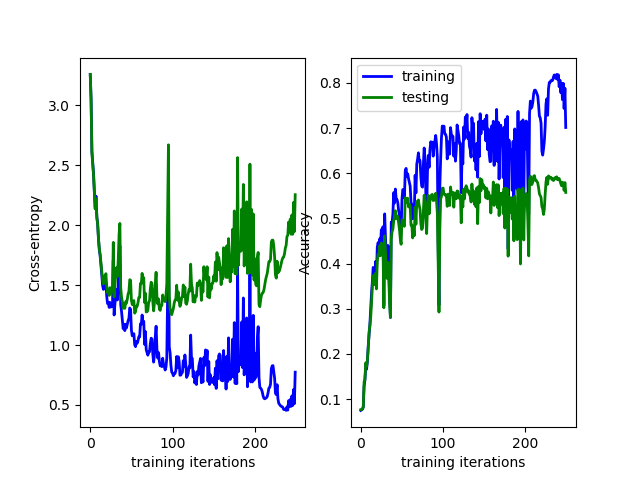
\includegraphics[width=\textwidth]{images/1relu0,001}
    \caption{0,001 learning rate ReLu}
  \end{minipage}
  \hfill
  \begin{minipage}[b]{0.4\textwidth}
    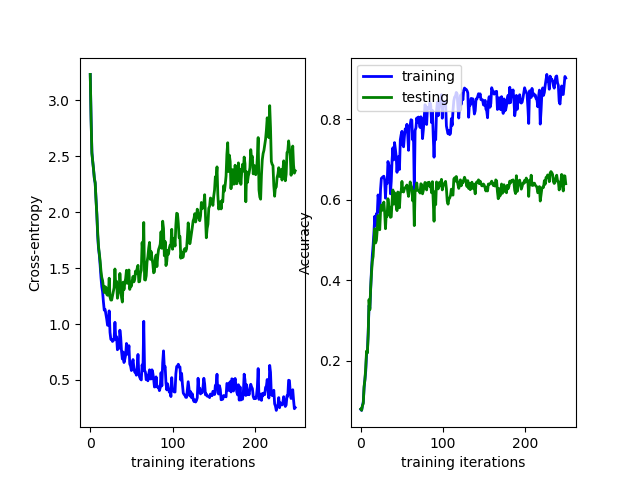
\includegraphics[width=\textwidth]{images/1relu0,002}
    \caption{Relu 0,002 learning rate}
  \end{minipage}
\end{figure}
\begin{figure}[H]
  \centering
  \begin{minipage}[b]{0.4\textwidth}
    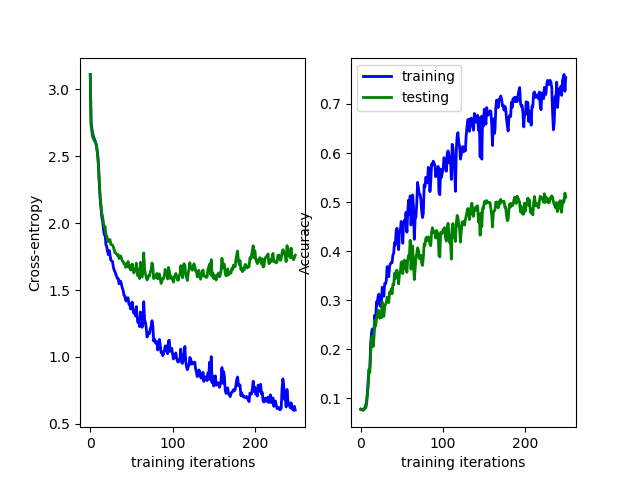
\includegraphics[width=\textwidth]{images/1tanh0,001}
    \caption{0,001 learning rate tanh}
  \end{minipage}
  \hfill
  \begin{minipage}[b]{0.4\textwidth}
    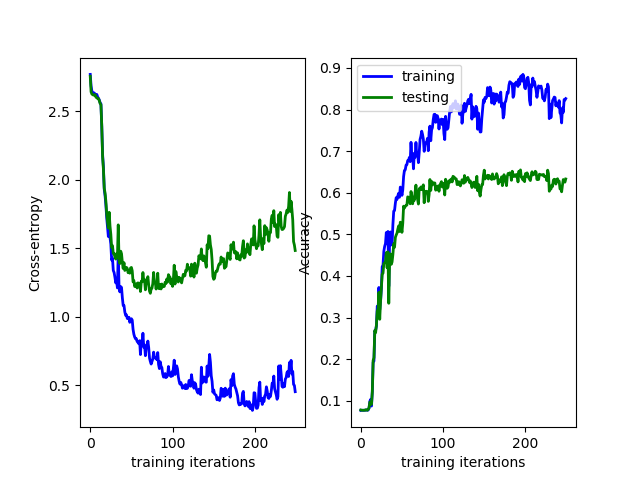
\includegraphics[width=\textwidth]{images/1tanh0,002}
    \caption{tanh 0,002 learning rate}
  \end{minipage}
\end{figure}
\end{document}
